\documentclass[document.tex]{subfiles} 

\begin{document}

\begin{comment}
\begin{savequote}[45mm]

من جد وجد ، ومن زرع حصد ، ومن سار على الدرب وصل.
\qauthor{مثل عربي}

\end{savequote}
\end{comment}

\chapter{المقاطعات \en{Interrupts}}
المقاطعات هي طريقة لإيقاف المعالج بشكل مؤقت من تنفيذ عملية ما (\en{Current Process}) والبدء بتنفيذ أوامر أخرى . وكمثال على ذلك هو عند الضغط على أي حرف في لوحة المفاتيح فان هذا يولد مقاطعة (\en{Interrupt}) تأتي كإشارة الى المعالج بأن يوقف ما يعمل عليه حاليا ويحفظ كل القيم التي يحتاجها لكي يستطيع مواصلة ما تم قطعه ، وفي حالة وجود دالة للتعامل مع هذه المقاطعة (مقاطعة لوحة المفاتيح) وتسمى دالة معالجة المقاطعة (\en{Interrupt Handler}) أو دالة خدمة المقاطعة (\en{Interrupt Service Rountine}) فان التنفيذ يتنقل اليها تلقائيا ، و يتم فيها معالجة هذه المقاطعة (مثلا يتم قراءة الحرف الذي تم ادخاله من متحكم لوحة المفاتيح ومن ثم ارساله الى متغير في الذاكرة) وعندما تنتهي دالة معالجة المقاطعة من عملها فان المعالج يعود ليُكْمِل تنفيذ العملية التي كان يعمل عليها. والمقاطعات إما تكون مقاطعات عتادية (\en{Hardware Interrupt}) وتصدر من عتاد الحاسب أو تكون برمجية (\en{Software Interrupt}) وتصدر من خلال البرامج عن طريق تعليمة \cmd{int n}. كذلك هناك مقاطعات يصدرها المعالج نفسه عند حدوث خطأ ما (مثلا عن القسمة على العدد صفر أو عند حدوث \en{Page Fault}) وتسمى هذه المقاطعات بأخطاء المعالج أو استثنائات المعالج (\en{Exceptions}) ويجب معالجة هذه الأخطاء (\en{Error Handler}) لأنها توقف عمل النظام في حالة لم تتوفر دالة لمعالجتها.


\section{المقاطعات البرمجية \en{Software Interrupts}}
المقاطعات البرمجية هي مقاطعات يتم اطلاقها من داخل البرنامج (عن طريق الأمر \cmd{int n}) لِنقل التنفيذ الى دالة أخرى تعالج هذه المقاطعة (\en{Interrupt handler})، وغالبا ما تستخدم هذه المقاطعات في برامج المستخدم (\en{Ring3 user mode}) للاستفادة من خدمات النظام (مثلا للقراءة والكتابة في أجهزة الإدخال والإخراج حيث لا توجد طريقة اخرى لذلك في نمط المستخدم).

\subsection{المقاطعات في النمط الحقيقي}
في النمط الحقيقي عندما يتم تنفيذ أمر المقاطعة (وهو ما يسمى بطلب تنفيذ المقاطعة (\en{Interrupt Request}) وتختصر بـ\en{IRQ})  فان المعالج يأخذ رقم المقاطعة المطلوب تنفيذها ويذهب بها الى جدول المقاطعات (\en{Interrupt Vector Table}) ، هذا الجدول يبدأ من العنوان الحقيقي \cmd{0x0} وينتهي عند العنوان \cmd{0x3ff} ويحوي كل سجل فيه على عنوان دالة معالجة المقاطعة (\en{IR}) والتي يجب تنفيذها لتخديم المقاطعة المطلوبة. حجم العنوان هو أربع بايت وتكون كالتالي:

\begin{english}
\begin{itemize}
\item \en{Byte 0: Low offset address of IR.}
\item \en{Byte 1: High offset address of IR.}
\item \en{Byte 2: Low Segment address of IR.}
\item \en{Byte 3: High Segment Address of IR.}
\end{itemize}
\end{english}

ويتكون الجدول من \cmd{256} مقاطعة (وبحسبة بسيطة يكون حجم الجدول هو \cmd{1024} بايت وهي ناتجة من ضرب عدد المقاطعات في حجم كل سجل )، بعض منها محجوز والبعض الاخر يستخدمه المعالج والبقية متروكة لمبرمج نظام التشغيل لدعم المزيد من المقطاعات. وبسبب أن الجدول يتكون فقط من عناوين لدوال معالجة المقاطعات فان هذا يمكننا من وضع الدالة في أي مكان على الذاكرة ومن ثم وضع عنوانها داخل هذا السجل (يتم هذا عن طريق مقاطعات البايوس)، والجدول التالي يوضح \en{IVT} والمقاطعات الموجودة فيه.

\begin{english}
\fontspec[Scale=1.2,Mapping=englishdigits]{Calibri}
\begin{tabular}{ | l | l | l |}
\hline  
Base Address & Interrupt Number & Description \\
\hline \hline
0x000	& 0 & Divide by 0 \\
0x004	& 1 & Single step (Debugger) \\
0x008	& 2 & Non Maskable Interrupt (NMI) Pin \\
0x00C	& 3 & Breakpoint (Debugger) \\
0x010	& 4 & Overflow \\
0x014	& 5 & Bounds check \\
0x018	& 6 & Undefined Operation Code \\
0x01C	& 7 & No coprocessor \\
0x020	& 8 & Double Fault \\
0x024	& 9 & Coprocessor Segment Overrun \\
0x028	& 10 & Invalid Task State Segment (TSS) \\
0x02C	& 11 & Segment Not Present \\
0x030	& 12 & Stack Segment Overrun \\
0x034	& 13 & General Protection Fault (GPF) \\
0x038	& 14 & Page Fault \\
0x03C	& 15 & Unassigned \\
0x040	& 16 & Coprocessor error \\
0x044	& 17 & Alignment Check (486+ Only) \\
0x048	& 18 & Machine Check (Pentium/586+ Only) \\
0x05C	& 19-31 & Reserved exceptions \\
0x068 - 0x3FF & 32-255 & Interrupts free for software use \\
 \hline  
\end{tabular}
\end{english}

\subsection{المقاطعات في النمط المحمي}
في النمط المحمي يستخدم المعالج جدولاً خاصاً يسمى بجدول واصفات المقاطعات (\en{Interrupt Descriptor Table}) ويختصر ب \en{IDT} ، هذا الجدول يشابه جدول \en{IVT} حيث يتكون من \cmd{256} واصفة كل واصفة مخصصة لمقاطعة ما (اذاً الجدول يحوي \cmd{256} مقاطعة) ، حجم كل واصفة هو \cmd{8} بايت  تحوي عنوان دالة معالجة المقاطعة (\en{IR}) و نوع الناخب (\en{selector type: code or data}) في جدول \en{GDT}  الذي تعمل عليه دالة معالجة المقاطعة ، بالاضافة الى مستوى الحماية المطلوب والعديد من الخصائص توضحها التركيبة التالية.

\begin{english}
\fontspec[Scale=1.2,Mapping=englishdigits]{Calibri}

\begin{itemize}
\item Bits 0-15:
\begin{itemize}
\item Interrupt / Trap Gate: Offset address Bits 0-15 of IR
\item Task Gate: Not used. 
\end{itemize}

\item Bits 16-31:
\begin{itemize}
\item Interrupt / Trap Gate: Segment Selector (Useually 0x10)
\item Task Gate: TSS Selector
\end{itemize}

\item Bits 31-35: Not used
\item Bits 36-38:
\begin{itemize}
\item Interrupt / Trap Gate: Reserved. Must be 0.
\item Task Gate: Not used.
\end{itemize}

\item Bits 39-41:
\begin{itemize}
\item Interrupt Gate: Of the format 0D110, where D determins size
\begin{itemize}
\item 01110 - 32 bit descriptor
\item 00110 - 16 bit descriptor
\end{itemize}
\item Task Gate: Must be 00101
\item Trap Gate: Of the format 0D111, where D determins size
\begin{itemize}
\item 01111 - 32 bit descriptor
\item 00111 - 16 bit descriptor
\end{itemize}

\end{itemize}

\item Bits 42-44: Descriptor Privedlge Level (DPL)
\begin{itemize}
\item 00: Ring 0
\item 01: Ring 1
\item 10: Ring 2
\item 11: Ring 3
\end{itemize}

\item Bit 45: Segment is present (1: Present, 0:Not present)
\item Bits 46-62: 
\begin{itemize}
\item Interrupt / Trap Gate: Bits 16-31 of IR address
\item Task Gate: Not used
\end{itemize}

\end{itemize}
\end{english}

والمثال التالي يوضح انشاء واصفة واحدة بلغة التجميع حتى يسهل تتبع القيم ، وسيتم كتابة مثال كامل لاحقا بلغة السي.

\begin{english}
\fontspec{Courier New}

\lstset{numberstyle=\tiny,numbers=left,stepnumber=1,numbersep=5pt,tabsize=2,extendedchars=true,breaklines=true,frame=b,showspaces=false, showtabs=false,xleftmargin=10pt,framexleftmargin=10pt,framexrightmargin=5pt,framexbottommargin=4pt,showstringspaces=false,language=[x86masm]Assembler}


\begin{lstlisting}[label=idt_desc,caption=\en{Example of interrupt descriptor}]

idt_descriptor:
   baseLow     	dw   0x0 
   selector      	dw   0x8
   reserved     	db   0x0 
   flags      	db   0x8e           ; 010001110
   baseHi      	dw   0x0

\end{lstlisting}
\end{english}

المتغير الأول \cmd{baseLow} هو أول \cmd{16} بت من عنوان دالة معالجة المقاطعة \en{IR} ويكمل الجزء الاخر من العنوان المتغير \cmd{baseHi} وفي هذا المثال العنوان هو \cmd{0x0} بمعنى أن دالة تخديم المقاطعة ستكون في العنوان \cmd{0x0}.  وبما أن دالة معالجة (تخديم) المقاطعة تحوي شفرة برمجية للتنفيذ وليست بيانات (\en{Data}) فان قيمة المتغير \cmd{selector} يجب أن تكون \cmd{0x8} للإشارة الى ناخب الشفرة (\en{Code Selector}) في جدول الواصفات العام (\en{GDT}).  أما المتغير \cmd{flags} فان قيمته هي \cmd{010001110b} دلالة على أن الواصفة هي \cmd{32-bit} وأن مستوى الحماية هو الحلقة صفر (\en{Ring0}).


وبعد أن يتم انشاء أغلب الواصفات بشكل متسلسل (في أي مكان على الذاكرة) ، يجب أن ننشئ جدول \en{IDT} وهذا يتم عن طريق حفظ عنوان أول واصفة في متغير وليكن \cmd{idt\_start} وعنوان نهاية الواصفات في المتغير \cmd{idt\_end} ومن ثم انشاء مؤشراً يسمى \cmd{idt\_ptr} والذي يجب أن يكون في صورة معينة بحيث يحفظ عنوان بداية الجدول ونهايته :

\begin{english}
\fontspec{Courier New}

\lstset{numberstyle=\tiny,numbers=left,stepnumber=1,numbersep=5pt,tabsize=2,extendedchars=true,breaklines=true,frame=b,showspaces=false, showtabs=false,xleftmargin=10pt,framexleftmargin=10pt,framexrightmargin=5pt,framexbottommargin=4pt,showstringspaces=false,language=[x86masm]Assembler}


\begin{lstlisting}[label=idt_ptr,caption=\en{Value to put in IDTR}]
idt_ptr:
	limit	dw idt_end - idt_start	; bits 0-15 is size of idt
	base	dd idt_start		; base of idt
\end{lstlisting}
\end{english}

هذا المؤشر يجب أن يتم تحميله الى المسجل \cmd{IDTR} (وهو مسجل داخل المعالج) عن طريق تنفيذ الامر \cmd{lidt}\footnote{بعد تنفيذ هذا الأمر فان جدول المقاطعات سيتم استبداله بالجدول الجديد والذي نجد عنوانه بداخل المسجل \cmd{idtr} ، وهذا الأمر لا يُنفَّذ إلاَّ  اذا كانت قيمة العلم (\en{CPL flag}) هي صفر.} بالشكل التالي \cmd{lidt [idt\_ptr]}.

وعند حدوث أي مقاطعة فان المعالج ينهي الأمر الذي يعمل عليه و يأخذ رقم المقاطعة ويذهب به الى جدول \en{IDT} (عنوان هذا الجدول يتواجد بداخل المسجل \en{IDTR}) ، وبعد ذلك يقوم بحساب مكان الواصفة بالمعادلة \cmd{int\_num * 8} وذلك بسبب أن حجم كل واصفة في جدول \en{IDT} هو \cmd{8} بايت. وقبل أن ينقل التنفيذ الى دالة معالجة المقاطعة فانه يجب أن يقوم بعملية حفظ للمكان الذي توقف فيه حتى يستطيع أن يتابع عمله عندما تعود دالة معالجة المقاطعة . ويتم حفظ الأعلام \cmd{EFLAGS} ومسجل مقطع الشفرة \cmd{CS} ومسجل عنوان التعليمة التالية \cmd{IP} في المكدس (\en{Stack})  الحالي ، وفي حالة حدوث خطأ ما فانه يتم دفع شفرة الخطأ (\en{Error Code}) الى المكدس أيضا. وشفرة الخطأ هي بطول \cmd{32-bit} وتتبع التركيبة التالية.

\begin{english}
\fontspec[Scale=1.2,Mapping=englishdigits]{Calibri}

\begin{itemize}
\item Bit 0: External event
\begin{itemize}
\item 0: Internal or software event triggered the error.
\item 1: External or hardware event triggered the error.
\end{itemize}
\item Bit 1: Description location
\begin{itemize}
\item 0: Index portion of error code refers to descriptor in GDT or current LDT.
\item 1: Index portion of error code refers to gate descriptor in IDT.
\end{itemize}
\item Bit 2: GDT/LDT. Only use if the descriptor location is 0.
\begin{itemize}
\item 0: This indicates the index portion of the error code refers to a descriptor in the current GDT.
\item 1: This indicates the index portion of the error code refers to a segment or gate descriptor in the LDT.
\end{itemize}
\item Bits 3-15: Segment selector index. This is an index into the IDT, GDT, or current LDT to the segment or gate selector bring refrenced by the error code.
\item  Bits 16-31: Reserved.

\end{itemize}
\end{english}

وعندما تنتهي دالة معالجة المقاطعة من عملها فانه يجب أن تنفذ الأمر \cmd{iret} أو \cmd{iretd} حتى يتم ارجاع القيم التي تم دفعها الى المكدس (قيم الأعلام \en{FLAGS}). وبالتالي يُكْمِل المعالج عمله.

 

\subsection{أخطاء المعالج}
خلال تنفيذ المعالج للأوامر فانه ربما يحدث خطأ ما مما يجعل المعالج يقوم بتوليد استثناء يعرف باستثناء المعالج ، ويوجد له عدة أنواع:

\begin{itemize}
\item الخطأ \en{Fault}: عندما تعمل دالة معالجة هذا النوع من الاستثناء فربما يتم اصلاح هذا الخطأ ، وعنوان العودة الذي يتم دفعه الى المكدس هو عنوان الأمر الذي تسبب في هذا الخطأ.
\item الخطأ \en{Trap}: عنوان العودة هو عنوان التعليمة التي تلي الأمر الذي تسبب في الخطأ.
\item الخطأ \en{Abort}: لا يوجد عنوان للعودة ، ولن يكمل البرنامج عمله بعد انتهاء دالة معالجة الخطأ. 
\end{itemize}

والجدول التالي يوضح أخطاء المعالج والمقاطعات التي يقوم بتوليدها.

% x86 Processor Exceptions Table.
\begin{english}
\fontspec[Scale=1.2,Mapping=englishdigits]{Calibri}
\begin{tabular}{ | l | l | l |}
\hline  
Interrupt Number & Class & Description \\
\hline \hline
0 & Fault & Divide by 0 \\
1 & Trap/Fault & Single step\\
2 & Unclassed & Non Maskable Interrupt (NMI) Pin \\
3 & Trap & Breakpoint\\
4 & Trap & Overflow \\
5 & Fault & Bounds check \\
6 & Fault & Unvalid OPCode \\
7 & Fault & Device not available \\
8 & Abort & Double Fault \\
9 & Abort & Coprocessor Segment Overrun \\
10 & Fault & Invalid Task State Segment\\
11 & Fault & Segment Not Present \\
12 & Fault & Stack Fault Exception \\
13 & Fault & General Protection Fault\\
14 & Fault & Page Fault \\
15 & -	& Unassigned \\
16 & Fault & x87 FPU Error \\
17 & Fault & Alignment Check \\
18 & Abort & Machine Check  \\
19 & Fault & SIMD FPU Exception \\
20-31 & - & Reserved \\
32-255 & - & Avilable for software use  \\
 \hline  
\end{tabular}
\end{english}

ويجدر بنا الوقوف على ملاحظة كنّا قد ذكرناها في الفصول السابقة وهي إلغاء المقاطعات (بواسطة الأمر \cmd{cli}) عند الانتقال الى النمط المحمي حتى لا يتسبب في حدوث خطأ \en{General Protection Fault} وبالتالي توقف النظام عن العمل وسبب ذلك هو أن عدم تنفيذ الأمر \cmd{cli} يعني أن المقاطعات العتادية مفعلة وبالتالي أي عتاد يمكنه أن يرسل مقاطعة الى المعالج لكي ينقل التنفيذ الى دالة تخديمها . وعند بداية الانتقال الى النمط المحمي فان جدول المقاطعات \en{IDT} لم يتم انشائه وأي محاولة لاستخدامه سيؤدي الى هذا الخطأ. أحد المتحكمات التي ترسل مقاطعات الى المعالج بشكل ثابت هو متحكم \en{Prpgrammable Interval Timer} وتختصر بمتحكم \en{PIT} وهي تمثل ساعة النظام \en{System Timer} بحيث ترسل مقاطعة بشكل دائم الى المعالج والذي بدوره ينقل التنفيذ الى دالة تخديم هذه المقاطعة . وبسبب أن جدول المقطاعات غير متواجد في بداية المرحلة الثانية من محمل النظام وكذلك لا توجد دالة لتخديم هذه المقاطعة فان هذا يؤدي الى توقف النظام ، لذلك يجب ايقاف المقاطعات العتادية لحين انشاء جدول المقطاعات وكتابة دوال معالجة المقاطعات. كذلك توجد مشكلة أخرى لبعض المقاطعات العتادية حيث انها تستخدم نفس أرقام المقاطعات التي يستخدمها المعالج للإستثناءات وحلها هو بإعادة برمجة الشريحة المسؤولة عن استقبال الاشارات من العتاد وتحويلها الى مقاطعات وارسالها الى المعالج ، هذه الشريحة تسمى \en{Programmable Interrupt Controller} وتختصر ب \en{PIC} ويجب إعادة برمجتها وتغيير ارقام المقاطعات للأجهزة التي تستخدم أرقاماً متشابهة.

وفيما يلي سيتم إنشاء جدول المقاطعات (\en{IDT}) باستخدام لغة السي وتوفير ال \cmd{256} دالة لمعالجة المقطاعات وحاليا سيقتصر عمل الدوال على طباعة رسالة ، وقبل ذلك سنقوم بانشاء جدول الواصفات العام (\en{GDT}) مجددا (أي سيتم الغاء الجدول الذي قمنا بانشائه في مرحلة الاقلاع) وبعد ذلك سنبدأ في برمجة متحكم \en{PIC} واعادة ترقيم مقاطعات الأجهزة وكذلك برمجة ساعة النظام لارسال مقاطعة بوقت محدد.  

\subsection{إنشاء جدول الواصفات العام \en{GDT}}
الهدف الرئيسي في نواة نظام التشغيل هي المحمولية على صعيد المنصات ، وهذا ما أدى الى اعتماد فكرة طبقة \en{HAL} والتي يقبع تحتها كل ما يتعلق بعتاد الحاسب وادارته وكل ما يجعل النظام معتمداً على معمارية معينة أيضا نجده تحت طبقة \en{HAL} ، وجدول الواصفات العام - كما ذكرنا في الفصول السابقة- يحدد ويقسم لنا الذاكرة الرئيسية كأجزاء قابلة للتنفيذ وأجزاء تحوي بيانات وغيرها ، ونظراً لأن إنشاء هذا الجدول يعتمد على معمارية المعالج والأوامر المدعومة فيه فانه يجب ان يقع تحت طبقة \en{HAL}\footnote{من منظور آخر هذه الجداول (\en{GDT,LDT and IDT}) هي جداول للمعالج لذلك يجب أن تكون في طبقة \en{HAL}.} وهذا يعني أن نقل النظام الى معمارية حاسوب آخر يتطلب فقط إعادة برمجة طبقة \en{HAL} .

بداية سنبدأ بتصميم الواجهة العامة لطبقة \en{HAL} ويجب أن نراعي أن تكون الواجهة مفصولة تماما عن التطبيق حتى يتمكن أي مطور من إعادة تطبيقها لاحقاّ على معمارية حاسوب آخر.

% HAL Layer
% kernel
% HAL [ device driver ]
% Hadrware

\begin{english}
\fontspec{Courier New}

\lstset{numberstyle=\tiny,numbers=left,stepnumber=1,numbersep=5pt,tabsize=2,extendedchars=true,breaklines=true,frame=b,showspaces=false, showtabs=false,xleftmargin=10pt,framexleftmargin=10pt,framexrightmargin=5pt,framexbottommargin=4pt,showstringspaces=false,language=C++}

\begin{lstlisting}[label=hal_interface,caption=\en{include/hal.h:Hardware Abstraction Layer Interface}]

#ifndef HAL_H
#define HAL_H

#ifndef i386
#error "HAL is not implemented in this platform"
#endif

#include <stdint.h>

#ifdef _MSC_VER
#define interrupt __declspec(naked)
#else
#define interrupt
#endif

#define far
#define near


/*	Interface	*/

extern int _cdecl hal_init();
extern int _cdecl hal_close();
extern void _cdecl gen_interrupt(int);


#endif // HAL_H
\end{lstlisting}
\end{english}

وحالياً واجهة طبقة \en{HAL} مكونة من ثلاث دوال تم الإعلان عنها بأنها \cmd{extern} وهذا يعني أن أي تطبيق (\en{Implementation}) لهذه الواجهة يجب أن يُعرِّف هذه الدوال. الدالة الاولى هي \cmd{hal\_init()} والتي تقوم بتهيئة العتاد وجداول المعالج بينما الدالة الثانية \cmd{hal\_close()} تقوم بعملية الحذف والتحرير وأخيرا الدالة \cmd{gen\_interrupt} والتي تم وضعها لغرض تجربة إرسال مقاطعة برمجية والتأكد من أن دالة معالجة المقاطعة تعمل كما يرام.

نعود بالحديث الى جدول الواصفات العام (\en{GDT}) \footnote{راجع \ref{sec:gdt}.} حيث سيتم انشائه بلغة السي وهذا ما سيسمح لنا باستخدام تراكيب عالية للتعبير عن الجدول و المؤشر مما يعطي وضوح ومقروئية أكثر في الشفرة.وسوف نحتاج  الى تعريف ثلاث دوال\footnote{لغرض التنظيم والتقسيم لا أكثر ولا أقل.}:

\begin{itemize}
\item الدالة \cmd{i386\_gdt\_init}: تقوم بتهيئة واصفة خالية وواصفة للشفرة وللبيانات وكذلك انشاء مؤشر الجدول.
\item الدالة \cmd{i386\_gdt\_set\_desc}: دالة تهيئة الواصفة حيث تستقبل القيم وتعينها الى الواصفة المطلوبة.
\item الدالة \cmd{gdt\_install}: تقوم بتحميل المؤشر الذي يحوي حجم الجدول وعنوان بدايته الى المسجل \en{GDTR}.  
\end{itemize}
والشفرة التالية توضح كيفية انشاء الجدول\footnote{راجع شفرة النظام لقراءة ملف الرأس \cmd{hal/gdt.h}.}.
\begin{english}
\fontspec{Courier New}

\lstset{numberstyle=\tiny,numbers=left,stepnumber=1,numbersep=5pt,tabsize=2,extendedchars=true,breaklines=true,frame=b,showspaces=false, showtabs=false,xleftmargin=10pt,framexleftmargin=10pt,framexrightmargin=5pt,framexbottommargin=4pt,showstringspaces=false,language=C++}

\begin{lstlisting}[label=gdt_c,caption=\en{hal/gdt.cpp:Install GDT}]

#include <string.h>
#include "gdt.h"
 
static struct gdt_desc _gdt[MAX_GDT_DESC];
static struct gdtr _gdtr;


static void gdt_install();


static void gdt_install() {
#ifdef _MSC_VER
	_asm lgdt [_gdtr];
#endif
}

extern void i386_gdt_set_desc(uint32_t index,uint64_t base,uint64_t limit,uint8_t access,uint8_t grand) {
	
	if ( index > MAX_GDT_DESC )
		return;
		
	// clear the desc.
	memset((void*)&_gdt[index],0,sizeof(struct gdt_desc));
	
	// set limit and base.
	_gdt[index].low_base = uint16_t(base & 0xffff);
	_gdt[index].mid_base = uint8_t((base >> 16) & 0xff);
	_gdt[index].high_base = uint8_t((base >> 24) & 0xff);
	_gdt[index].limit = uint16_t(limit & 0xffff);
	
	// set flags and grandularity bytes
	_gdt[index].flags = access;
	_gdt[index].grand = uint8_t((limit >> 16) & 0x0f);
	_gdt[index].grand = _gdt[index].grand | grand & 0xf0;
}

extern gdt_desc* i386_get_gdt_desc(uint32_t index) {
	if ( index >= MAX_GDT_DESC )
		return 0;
	else
		return &_gdt[index];
}

extern int i386_gdt_init() {
	
	// init _gdtr
	_gdtr.limit = sizeof(struct gdt_desc) * MAX_GDT_DESC - 1;
	_gdtr.base = (uint32_t)&_gdt[0];
	
	// set null desc.
	i386_gdt_set_desc(0,0,0,0,0);
	
	// set code desc.
	i386_gdt_set_desc(1,0,0xffffffff,
		I386_GDT_CODE_DESC|I386_GDT_DATA_DESC|I386_GDT_READWRITE|I386_GDT_MEMORY, 	// 10011010
		I386_GDT_LIMIT_HI|I386_GDT_32BIT|I386_GDT_4K 								// 11001111
 
	);
	
	// set data desc.
	i386_gdt_set_desc(2,0,0xffffffff,
		I386_GDT_DATA_DESC|I386_GDT_READWRITE|I386_GDT_MEMORY, 	// 10010010
		I386_GDT_LIMIT_HI|I386_GDT_32BIT|I386_GDT_4K			// 11001111
	);
	
	// install gdtr
	gdt_install();
	
	return 0;
}

\end{lstlisting}
\end{english}

\subsection{إنشاء جدول المقاطعات \en{IDT}}
% يكمل لاحقا..

\section{متحكم المقاطعات القابل للبرمجة \en{Programmable Interrupt Controller}}
السبب الرئيسي في تعطيل المقاطعات العتادية عند الإنتقال الى النمط المحمي (\en{PMode}) هو بسبب عدم توفر دوال لمعالجة المقاطعات في تلك اللحظة ، وحتى لو قمنا بتوفير ال 256 دالة لمعالجة المقاطعات فان هنالك مشكلة استخدام نفس رقم المقاطعة لأكثر من غرض ، فمثلا مؤقتة النظام \en{PIT} التي ترسل مقاطعات بشكل دائم تستخدم المقاطعة رقم 8 والتي هي أيضا أحد استثناءات المعالج ، لذلك في كلتا الحالات سيتم استدعاء دالة تخديم واحدة وهو شيء مرفوض تماماً. لذلك الحل الوحيد هو بإعادة برمجة المتحكم المسؤول عن استقبال الإشارات من متحكمات العتاد  وتعيين أرقام مختلفة بخلاف تالك الأرقام التي يستخدمها المعالج للأخطاء والاستثناءات ، هذا المتحكم (انظر الشكل \ref{fig:pic}) وظيفته هي استقبال إشارات من متحكمات العتاد ومن ثم يقوم بتحويلها الى أرقام مقاطعات تُرسل بعد ذلك الى المعالج الذي يقوم بنقل التنفيذ اليها ، ويعرف هذا المتحكم بمتحكم \en{PIC} اختصاراً ل \en{Programmable Interrupt Controller} ويعرف أيضا بالإسم \en{8259A} ، وفي هذا البحث سنستخدم المسمى متحكم \en{PIC}.

% يجب شرح Level Triggered Mode and Edge Triggered Mode 
\begin{figure}[h!]
  \label{fig:pic} 
  \caption{متحكم المقاطعات القابل للبرمجة \en{8259A}}
  \centering
   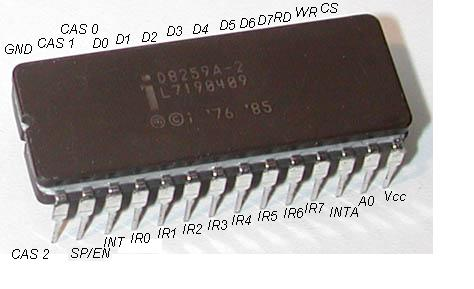
\includegraphics[width=0.5\textwidth]{../img/Intel-D8259A}
\end{figure}


\subsection{المقاطعات العتادية \en{Hardware Interrupts}}
قبل أن نبدأ في الدخول في تفاصيل متحكم \en{PIC} يجب إعطاء نبذة عن المقاطعات العتادية حيث ذكرنا أنها مقاطعات تختلف عن المقاطعات البرمجية من ناحية أن مصدرها يكون من العتاد وليس من برنامج ما ، وهذا ما أدى الى ظهور لقب مسير للأحداث (\en{Interrupt Driven}) على أجهزة الحاسب. حيث قديما لم يكن هناك طريقة للتعامل مع العتاد إلا باستخدام حلقة برمجية (\en{loop}) على مسجل ما في متحكم العتاد حتى تتغير قيمته دلالة على أن هناك قيمة أو نتيجة قد جاءت من العتاد ، هذه الطريقة في التخاطب مع العتاد تسمى \en{Polling}\footnote{وتسمى أيضا ب \en{Busy Waiting}.} وهي تضيع وقت المعالج في انتظار قيمة لا يُعرف هل ستظهر أم لا  وقد تم إلغائها في التخاطب مع العتاد حيث الان أصبح أي متحكم عتاد يدعم إرسال الإشارات (وبالتالي المقاطعات) الى المعالج والذي قد يعمل على عملية أخرى ، وهكذا تم الإستفادة من وقت المعالج وأصبح التخاطب هو غير متزامن (\en{Asynchronous}) بدلاً من متزامن (\en{Synchronous}). وعندما يبدأ الحاسب في الإقلاع فان نظام البايوس يقوم بترقيم عتاد الحاسب وإعطاء رقم مقاطعة لكل متحكم وبسبب تكرار هذه الأرقام فانه يجب تغييرها لأرقام أخرى وهذا يتم بسهولة في النمط الحقيقي وذلك باستخدام مقاطعات البايوس أما في النمط المحمي فيجب أن نقوم بالتخاطب المباشر مع المتحكم الذي لديه أرقام المقاطعات ومن ثم تغييرها . والجدول \ref{tbl:irq} يوضح أرقام المقاطعات لمتحكمات الحاسب.

\begin{table}
\caption{مقاطعات العتاد لحواسيب \en{x86}}
\centering
\begin{tabular}{ | r | r | r |}
\hline  
رقم المشبك(الدبوس) & رقم المقاطعة & الوصف \\
\hline \hline
\en{IRQ0} & \en{0x08} & المؤقتة \en{Timer} \\
\en{IRQ1} & \en{0x09} & لوحة المفاتيح \\
\en{IRQ2} & \en{0x0a} & يُربط مع متحكم \en{PIC} ثانوي \\
\en{IRQ3} & \en{0x0b} & المنفذ التسلسلي 2 \\
\en{IRQ4} & \en{0x0c} & المنفذ التسلسلي 1 \\
\en{IRQ5} & \en{0x0d} & منفذ التوازي 2 \\
\en{IRQ6} &\en{0x0e} & متحكم القرص المرن \\
\en{IRQ7} & \en{0x0f} & منفذ التوازي 1 \\
\en{IRQ8/IRQ0} & \en{0x70} & ساعة ال \en{CMOS} \\
\en{IRQ9/IRQ1} & \en{0x71} &  \en{CGA vertical retrace} \\
\en{IRQ10/IRQ2} & \en{0x72} & محجوزة \\
\en{IRQ11/IRQ3} & \en{0x73} & محجوزة \\
\en{IRQ12/IRQ4} & \en{0x74} & محجوزة \\
\en{IRQ13/IRQ5} & \en{0x75} & وحدة \en{FPU} \\
\en{IRQ14/IRQ6} & \en{0x76} & متحكم القرص الصلب \\
\en{IRQ15/IRQ7} & \en{0x77} & محجوزة \\
 \hline  
\end{tabular}
\label{tbl:irq}
\end{table}

\subsection{برمجة متحكم \en{PIC}}
متحكم \en{PIC} يستقبل إشارات (\en{Signals}) من متحكمات العتاد والتي تكون موصولة به ومن ثم يقوم بتحويلها الى أرقام مقاطعات لكي يقوم المعالج بنقل التنفيذ الى دالة تخديمها ، ويراعي متحكم \en{PIC} أولية متحكمات العتاد ، فمثلا لو تم إرسال إشارتين في نفس الوقت الى متحكم \en{PIC} فان المتحكم سوف يراعي الأولية ويقوم بارسال رقم مقاطعة العتاد ذو الأولية أولا وبعد أن تنتهي دالة تخديم المقاطعة يقوم المتحكم بارسال الرقم الآخر . ونظراً لتعقيدات بناء المتحكم فانه يتعامل فقط مع 8 أجهزة مختلفة (أي 8 مقاطعات \en{IRQ}) وهذا ما أدى مصنعى الحاسب الى توفير متحكم \en{PIC} آخر يعرف بالمتحكم الثانوي (\en{Secondary/Slave PIC}) . المتحكم الرئيسي (\en{Primary PIC}) يوجد داخل المعالج ويرتبط مع المتحكم الثانوي والذي يتواجد في الجسر الجنوبي (\en{SouthBridge}) .

\subsubsection{مشابك المتحكم \en{PIC's Pins}}
تعتبر مشابك المتحكم هي  طريقة ارسال البيانات من المتحكم الى المعالج (أو الى متحكم رئيسي) ، ونظراً لان كل مشبك لديه وظيفة محددة فانه يجب دراسة هذه المشابك ولكن لن نفصِّل كثيراً حيث أن الموضوع متشعب ويخص دراسي المنطق الرقمي (\en{Digital Logic}). ويوضح الشكل \ref{pic_pins} هذه المشابك.

\begin{wrapfigure}{l}{0.5\textwidth}
\label{fig:pic_pins} 
  \vspace{-20pt}
  \begin{center}
    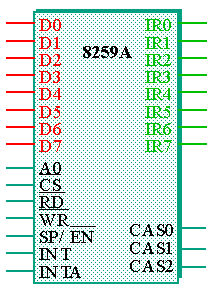
\includegraphics[width=0.48\textwidth]{../img/pic_pins}
  \end{center}
  \vspace{-20pt}
  \caption{مشابك متحكم \en{PIC}}
  \vspace{-10pt}
\end{wrapfigure}

حيث أن المشابك \en{D0-D7} هي لإرسال البيانات الى متحكم \en{PIC} أما المشابك \en{CAS0, CAS1, CAS2} تستخدم للتخاطب بين متحكمات \en{PIC} الرئيسية والثانوية ، والمشبك \en{INT} يرتبط مع مشبك للمعالج وهو \en{INTR} كذلك المشبك \en{INTA} يرتبط مع مشبك المعالج \en{INTA} وهذه المشابك لها العديد من الفوائد حيث عندما يقوم المعالج بتنفيذ أي مقاطعة فانه يقوم بتعطيل قيم العلمين \en{IF and TF} وهذا ما يجعل مشبك المعالج \en{INTR} يغلق مباشرة وبالتالي لا يمكن لمتحكم \en{PIC} إرسال أي مقاطعة عبر مشبكه \en{INT} حيث أن الجهة المقابلة لها تم غلقها وبالتالي لا يمكن لمقاطعة أن تقطع مقاطعة أخرى وإنما يتم حجرها في مسجل داخل \en{PIC} الى أن ينتهي المعالج من تنفيذ المقاطعة والعودة بإشارة (تسمى إشارة نهاية المقاطعة \en{End Of Interrupt}) تدل على أن المقاطعة قد انتهت. أخيرا ما يهمنا في هذه المشابك هي مشابك \en{IR0...IR7} وهي مشابك ترتبط مع متحكمات العتاد المراد استقبال الإشارات منه عند حدوث شيء معين (الضغط على حرف في لوحة المفاتيح مثلاً) ويمكن لهذه المشابك أن ترتبط مع متحكمات \en{PIC} أخرى ولا يوجد شرط ينص على وجوب توفر متحكمين \en{PIC} وإنما يمكن ربط كل مشبك من هذه المشابك الثمانية مع متحكم \en{PIC} وهكذا سيتواجد 8 متحكمات تدعم حتى 256 مقاطعة عتادية مختلفة. ويجب ملاحظة أن متحكم العتاد الذي يرتبط بأول مشبك \en{IR0} لديه الأولية الأولى في التنفيذ وهكذا على التوالي.\\

\subsubsection{مسجلات متحكم \en{PIC}}
يحوي متحكم \en{PIC} على عدة مسجلات داخلية وهي:

\begin{itemize}
\item مسجل الأوامر (\en{Command Reigster}): ويستخدم لإرسال الأوامر الى المتحكم ، وهناك عدد من الأوامر مثل أمر القراءة من مسجل ما أو أمر ارسال اشارة \en{EOI}.
\item  مسجل الحالة (\en{Status Register}): وهو مسجل للقراءة فقط حيث تظهر عليه حالة المتحكم.
\item مسجل طلبات المقاطعات (\en{Interrupt Request Register}):  يحفظ هذا المسجل الأجهزة التي طلبت تنفيذ مقاطعتها وهي بانتظار وصول إشعار (\en{Acnowledges}) من المعالج ، والجدول \ref{tbl:irr} يوضح بتات هذا المسجل.

\begin{table}
\caption{مسجل \en{IRR/ISR/IMR}}
\centering
\begin{tabular}{ | r | r | r |}
\hline  
 \en{Bit Number} &  \en{IRQ Number (Primary controller)} & \en{IRQ Number (Slave controller)}   \\
\hline \hline
\en{0} & \en{IRQ0} & \en{IRQ8}  \\
\en{1} & \en{IRQ1} & \en{IRQ9} \\
\en{2} & \en{IRQ2} & \en{IRQ10} \\
\en{3} & \en{IRQ3} & \en{IRQ11}\\
\en{4} & \en{IRQ4} & \en{IRQ12} \\
\en{5} & \en{IRQ5} & \en{IRQ13} \\
\en{6} & \en{IRQ6} &\en{IRQ14}  \\
\en{7} & \en{IRQ7} & \en{IRQ15}   \\
 \hline  
\end{tabular}
\label{tbl:irr}
\end{table}
وفي حالة كانت قيمة أي بت هي 1 فهذا يعني أن متحكم العتاد بانتظار الإشعار من المعالج.

\item مسجل الخدمة (\en{In Service Register (ISR)}): يدل على المسجل على أن طلب المقاطعة قد نجح وأن الإشعار قد وصل لكن لم تنتهي دالة تخديم المقاطعة من عملها. 

\item مسجل (\en{Interrupt Mask Register (IMR)}): يحدد هذا المسجل ما هي المقاطعات التي يجب تجاهلها وعدم ارسال إشعار لها وذلك حتى يتم التركيز على المقاطعات الأهم.
\end{itemize}

والجدول \ref{tbl:pic_port} يوضح عناوين منافذ المسجلات في حواسيب \en{x86}.

\begin{table}
\caption{عناوين المنافذ لمتحكم \en{PIC}}
\centering
\begin{tabular}{ | l | l |}
\hline  
 رقم المنفذ &  الوصف  \\
\hline \hline
\en{0x20} & \en{Primary PIC Command and Status Register}\\
\en{0x21} & \en{Primary PIC Interrupt Mask Register and Data Register}\\
\en{0xA0} & \en{Secondary (Slave) PIC Command and Status Register} \\
\en{0xA1} & \en{Secondary (Slave) PIC Interrupt Mask Register and Data Register}\\
 \hline  
\end{tabular}
\label{tbl:pic_port}
\end{table}


\subsubsection{برمجة متحكم \en{PIC}}
لبرمجة متحكم \en{PIC} وإعادة ترقيم المقاطعات فإن ذلك يتطلب إرسال بعض الأوامر الى المتحكم بحيث تأخذ هذه الأوامر نمط معين تُحَدَّد بها عمل المتحكم. وتوجد أريع أوامر يجب إرسالها لهذا الغرض تعرف ب \en{Initialization Control Words} وتختصر بأوامر تهيئة \en{ICW} . وفي حالة توفر أكثر من متحكم \en{PIC} على النظام فيجب أن تُرسل هذه الأوامر الى المتحكم الآخر كذلك. \textbf{الأمر الأول \en{ICW1}} وهو الأمر الرئيسي والذي يجب إرساله أولا الى المتحكم الرئيسي والثانوي ويأخذ 7 بتات ويوضح الجدول \ref{tbl:icw1} هذه البتات ووظيفة كل بت.

\begin{table}
\caption{الأمر الأول \en{ICW1}}
\centering
\begin{tabular}{ | r | r | r |}
\hline  
 رقم البت & القيمة & الوصف   \\
\hline \hline
\en{0} & \en{IC4} & إرسال الأمر \en{ICW4}  \\
\en{1} & \en{SNGL} & هل يوجد متحكم \en{PIC} واحد \\
\en{2} & \en{ADI} & تأخذ القيمة صفر في حواسيب \en{x86} \\
\en{3} & \en{LTIM} & نمط عمل المقاطعة\\
\en{4} & \en{1} & بت التهيئة \\
\en{5} & \en{0} &  تأخذ القيمة صفر في حواسيب \en{x86} \\
\en{6} & \en{0} &  تأخذ القيمة صفر في حواسيب \en{x86}  \\
\en{7} & \en{0} & تأخذ القيمة صفر في حواسيب \en{x86}   \\
 \hline  
\end{tabular}
\label{tbl:icw1}
\end{table}
حيث أن البت الأول يحدد ما اذا كان يجب إرسال أمر التحكم \en{ICW4} أم لا وفي حالة كان قيمة البت هي 1 فإنه يجب إرسال الأمر \en{ICW4} أما البت الثاني فغالباً يأخذ القيمة صفر دلالة على أن هناك أكثر من متحكم \en{PIC} في النظام ، والبت الثالث غير مستخدم أما الرابع فيحدد نمط عمل المقاطعة هل هي \en{Level Triggered Mode} أم \en{Edge Triggered Mode} ، أما البت الخامس فيجب أن يأخذ القيمة 1 دلالة على أننا سنقوم بتهيئة متحكم \en{PIC} وبقية البتات غير مستخدمة في حواسيب \en{x86}. والشفرة \ref{icw1}  توضح إرسال الأمر الأول الى متحكم \en{PIC} الرئيسي والثانوي.

\begin{english}
\fontspec{Courier New}

\lstset{numberstyle=\tiny,numbers=left,stepnumber=1,numbersep=5pt,tabsize=2,extendedchars=true,breaklines=true,frame=b,showspaces=false, showtabs=false,xleftmargin=10pt,framexleftmargin=10pt,framexrightmargin=5pt,framexbottommargin=4pt,showstringspaces=false,language=[x86masm]Assembler}


\begin{lstlisting}[label=icw1,caption=\en{Initialization Control Words 1}]
	; Setup to initialize the primary PIC. Send ICW 1
	mov	al, 0x11               ; 00010001
	out	0x20, al
 
	 ; Send ICW 1 to second PIC command register
	out	0xA0, al
\end{lstlisting}
\end{english}

\textbf{الأمر الثاني \en{ICW2}} يستخدم لإعادة تغيير عنواين جدول \en{IVT} الرئيسية للطلبات المقاطعات \en{IRQ} وبالتالي عن طريق هذا الأمر يمكن أن نغير أرقام المقاطعات لل \en{IRQ} الى أرقام أخرى . ويجب أن يرسل هذا الأمر مباشرة بعد الأمر الأول كذلك يجب أن يتم اختيار أرقاما غير مستخدمة من قبل المعالج حتى لا نقع في نفس المشكلة السابقة ( وهي أكثر من \en{IRQ} يستخدم نفس رقم المقاطعة وبالتالي لديهم دالة تخديم واحدة). والمثال \ref{icw2} يوضح كيفية تغيير أرقام \en{IRQ} لمتحكم \en{PIC} الرئيسي والثانوي بحيث يتم استخدام أرقام المقاطعات 32-39 للمتحكم الأول والأرقام من 40-47 للمتحكم الثانوي وهي أرقاماً خالية لا يستخدمها المعالج وتقع مباشرة بعد آخر مقاطعة للمعالج الذي يستخدم 32 مقاطعة بدءاً من الصفر وانتهاءاً بالمقاطعة 31.
\begin{english}
\fontspec{Courier New}

\lstset{numberstyle=\tiny,numbers=left,stepnumber=1,numbersep=5pt,tabsize=2,extendedchars=true,breaklines=true,frame=b,showspaces=false, showtabs=false,xleftmargin=10pt,framexleftmargin=10pt,framexrightmargin=5pt,framexbottommargin=4pt,showstringspaces=false,language=[x86masm]Assembler}


\begin{lstlisting}[label=icw2,caption=\en{Initialization Control Words 2}]
	; send ICW 2 to primary PIC
	mov	al, 0x20		
	out	0x21, al
	; Primary PIC handled IRQ 0..7. IRQ 0 is now mapped to interrupt number 0x20
	
	
	; send ICW 2 to secondary PIC
	mov	al, 0x28		
	out	0xA1, al
	; Secondary PIC handles IRQ's 8..15. IRQ 8 is now mapped to use interrupt 0x28
\end{lstlisting}
\end{english}

\textbf{الأمر الثالث \en{ICW3}} يستخدم في حالة كان هناك أكثر من متحكم \en{PIC} حيث يجب أن نحدد رقم طلب المقاطعة \en{IRQ} التي يستخدمها المتحكم الثانوي للتخاطب مع المتحكم الرئيسي. وفي حواسيب \en{x86} غالباً ما يستخدم \en{IRQ2} لذا يجب إرسال هذا الأمر الى المتحكم، لكن كل متحكم يتوقع الأمر بصيغة معينة يوضحها الجدولان \ref{tbl:icw_ppic} و \ref{tbl:icw_spic} .

\begin{table}
\caption{الأمر الثالث للمتحكم الرئيسي \en{ICW3 for Primary PIC}}
\centering
\begin{tabular}{ | r | r | r |}
\hline  
رقم البت & القيمة & الوصف \\
\hline \hline
\en{0-7} & \en{S0-S7} & رقم \en{IRQ} التي يتصل بها المتحكم الثانوي  \\
 \hline  
\end{tabular}
\label{tbl:icw_ppic}
\end{table}

\begin{table}
\caption{الأمر الثالث للمتحكم الثانوي \en{ICW3 for Slave PIC}}
\centering
\begin{tabular}{ | r | r | r |}
\hline  
 رقم البت & القيمة & الوصف   \\
\hline \hline
\en{0-2} & \en{ID0} & رقم \en{IRQ} التي يتصل بها مع المتحكم الرئيسي  \\
\en{3-7} & \en{3-7} & محجوزة  \\
 \hline  
\end{tabular}
\label{tbl:icw_spic}
\end{table}

ويجب إرسال الأمر بحسب الصيغة التي يقبلها مسجل البيانات للمتحكم ، فمتحكم \en{PIC} الرئيسي يستقبل رقم \en{IRQ} على شكل 7 بت بحيث يتم تفعيل رقم البت المقابل لرقم \en{IRQ} وفي مثالثا يرتبط المتحكم الرئيسي مع الثانوي عبر \en{IRQ2} لذلك يجب تفعيل قيمة البت 2 (أي يجب إرسال القيمة \en{0000100b} وهي تعادل \en{0x4})  بينما المتحكم الثانوي يقبل رقم \en{IRQ} عن طريق إرسال قيمته على الشكل الثنائي وهي 2 (وتعادل بالترميز الثنائي \en{010}) وبقية البتات محجوزة (انظر جدول \ref{tbl:icw_spic}) ، والمثال \ref{icw3} يوضح كيفية إرسال الأمر الثالث الى المتحكمين.

\begin{english}
\fontspec{Courier New}

\lstset{numberstyle=\tiny,numbers=left,stepnumber=1,numbersep=5pt,tabsize=2,extendedchars=true,breaklines=true,frame=b,showspaces=false, showtabs=false,xleftmargin=10pt,framexleftmargin=10pt,framexrightmargin=5pt,framexbottommargin=4pt,showstringspaces=false,language=[x86masm]Assembler}


\begin{lstlisting}[label=icw3,caption=\en{Initialization Control Words 3}]
	; Send ICW 3 to primary PIC
	mov	al, 0x4		; 0x04 => 0100, second bit (IR line 2)
	out	0x21, al	; write to data register of primary PIC
 
	; Send ICW 3 to secondary PIC
	mov	al, 0x2		; 010=> IR line 2
	out	0xA1, al	; write to data register of secondary PIC
\end{lstlisting}
\end{english}

\textbf{الأمر الرابع \en{ICW4}} هو آخر أمر تحكم يجب إرساله الى المتحكمين ويأخذ التركيبة التي يوضحها جدول \ref{tbl:icw4}.

\begin{table}
\caption{الأمر الرابع \en{ICW4}}
\centering
\begin{tabular}{ | r | r | r |}
\hline  
 رقم البت & القيمة & الوصف   \\
\hline \hline
\en{0} & \en{uPM} & يجب تفعيل هذا البت في حواسيب \en{x86} \\
\en{1} & \en{AEOI} & جعل المتحكم يقوم بإرسال إشارة \en{EOI} \\
\en{2} & \en{M/S} &  \en{If set (1), selects buffer master. Cleared if buffer slave.} \\
\en{3} & \en{BUF} & \en{If set, controller operates in buffered mode}\\
\en{4} & \en{SFNM} & تأخذ القيمة صفر في حواسيب \en{x86}  \\
\en{5-7} & \en{0} &  تأخذ القيمة صفر في حواسيب \en{x86} \\
 \hline  
\end{tabular}
\label{tbl:icw4}
\end{table}
وفي الغالب لا يوجد حوجة لتفعيل كل هذه الخصائص ، فقط أول بت يجب تفعيله حيث يستخدم مع حواسيب \en{x86} . والمثال \ref{icw4} يوضح كيفة إرسال الأمر الرابع الى المتحكم \en{PIC} الرئيسي والثانوي.

\begin{english}
\fontspec{Courier New}

\lstset{numberstyle=\tiny,numbers=left,stepnumber=1,numbersep=5pt,tabsize=2,extendedchars=true,breaklines=true,frame=b,showspaces=false, showtabs=false,xleftmargin=10pt,framexleftmargin=10pt,framexrightmargin=5pt,framexbottommargin=4pt,showstringspaces=false,language=[x86masm]Assembler}


\begin{lstlisting}[label=icw4,caption=\en{Initialization Control Words 4}]
	mov	al, 1		; bit 0 enables 80x86 mode
 
	; send ICW 4 to both primary and secondary PICs
	out	0x21, al
	out	0xA1, al
\end{lstlisting}
\end{english}

وبعد إرسال هذه الأوامر الأربع تكتمل عملية تهيئة متحكم \en{PIC} الرئيسي والثانوي ، وفي حالة حدوث أي مقاطعة من متحكم لعتاد ما ، فإن أرقام المقاطعات التي سترسل الى المعالج هي الأرقام التي قمنا بتعيينها في الأمر الثاني (وتبدأ من 32 الى 47) وهي تختلف بالطبع عن الأرقام التي يستخدمها المعالج.

 
\subsubsection{كيف تعمل مقاطعات العتاد}
عندما يحتاج متحكم أي عتاد لفت انتباه المعالج الى شيء ما فأول خطوة يقوم بها هي إرسال إشارة الى متحكم \en{PIC} (وعلى سبيل المثال سنفرض أن هذا المتحكم هو متحكم المؤقتة \en{PIT} والتي ترتبط بالمشبك \en{IR0}) هذه الإشارة ترسل عبر مشبك \en{IR0} ، حينها يقوم متحكم \en{PIC} بتسجيل طلب المتحكم \en{IRQ} في مسجل يسمى مسجل طلبات المقاطعات (\en{Interrupt Request Register}) ويعرف اختصاراً بمسجل \en{IRR} . هذا المسجل بطول 8 بت كل بت فيه يمثل رقم \en{IRQ} ويتم تفعيل أي بت عند طلب مقاطعة من المتحكم ، وفي مثالنا سيتم تفعيل البت \en{0} بسبب أن المؤقتة ترتبط مع \en{IR0}. بعد ذلك يقوم متحكم \en{PIC} بفحص مسجل \en{Interrupt Mask Register} ليتأكد من أنه لا توجد هناك مقاطعة ذات أولية أعلى حيث في هذه الحالة على المقاطعة الجديدة أن تننظر حتى يتم تخديم كل المقاطعات ذات الأولوية. وبعد ذلك يُرسل \en{PIC} إشارة الى المعالج من خلال مشبك \en{INTA} لأخبار المعالج بأن هناك مقاطعة يجب تنفيذها. وهنا يأتي دور المعالج حيث يقوم بالإنتهاء من تنفيذ الأمر الحالي الذي يعمل عليه ومن ثم يقوم بفحص قيمة العلم \en{IF} حيث في حالة كانت غير مفعلة فان المعالج سوف يتجاهل طلب تنفيذ المقاطعة، أما إذا وجد المعالج قيمة العلم مفعلة فانه يقوم بارسال إشعار (\en{Acnowledges}) عبر مشبك \en{INTR} الى متحكم \en{PIC} الذي بدوره يستقبلها من مشبك \en{INTA} ويضع رقم المقاطعة ورقم \en{IRQ} في المشابك \en{D0-D7} ، وأخيرا يفعل قيمة البت 0 في مسجل \en{In Service Register} دلالة على أن مقاطعة المؤقتة جاري تنفيذها. وعندما يحصل المعالج على رقم المقاطعة فانه يقوم بوقف العملية التي يعمل عليها ويحفظ قيم مسجل الأعلام ومسجل \en{CS and EIP} وإذا كان المعالج يعمل في النمط الحقيقي فإنه يأخذ رقم المقاطعة ويذهب بها كدليل الى جدول المقطاعات \en{IVT} حيث يجد عنوان دالة تخديم المقاطعة ومن ثم ينقل التنفيذ اليها ، أما اذا كان المعالج يعمل في النمط المحمي فانه يأخذ رقم المقاطعة ويذهب بها الى جدول واصفات المقاطعات حيث يجد دالة تخديم المقاطعة. وعندما تنتهي دالة تخديم المقاطعة من عملها فانها يجب أن ترسل إشارة \en{EOI} حتى يتم تفعيل المقاطعات مجدداً.



\section{المؤقتة \en{Programmable Interval Timer}}
المؤقتة هي شريحة \en{Dual Inline Package (DIP)} تحوي ثلاث عدادات (\en{Counters or Channels}) تعمل كمؤقتات لإدارة ثلاث أشياء (انظر الشكل \ref{fig:pit}). العداد الأول ويُعرف \textbf{بمؤقت النظام (\en{System Timer})} وظيفته ارسال طلب مقاطعة (\en{IRQ0}) الى متحكم \en{PIC} وذلك لتنفيذ مقاطعة ما كل فترة محددة ، هذه الفترة يتم تحديدها عند برمجة هذه المؤقتة ويُستفاد من هذه المؤقتة في عملية تزامن العمليات وتوفير بنية تحتية لمفهوم تعدد العمليات والمسالك (\en{Multitask and Multithread}) حيث أن الفترة التي تقوم بها مؤقتة النظام لاصدار طلب المقاطعة سيكون هو الوقت المحدد لأي عملية (\en{Process}) موجودة في طابور العمليات (\en{Process Queue}) وبعد ذلك ترُسل العملية الى آخر الصف في حالة لم تنتهي من عملها بعد ويبدأ المعالج في تنفيذ العملية التالية تحت نفس الفترة المحددة.  أما العداد الثاني فيُستخدم في \textbf{عملية تنعيش الذاكرة الرئيسية (\en{RAM refreshing})} حتى تحافظ على محتوياتها من الفقدان أثناء عمل الحاسب ويجدر بنا ذكر أن هذه المهمة قد أُحيلت الى متحكم الذاكرة (\en{Memory Controller}) وأصبحت هذه المؤقتة لا تستخدم في العادة. أما العداد الأخير فيستخدم في عملية \textbf{إرسال الصوت الى سماعات الحاسب}\footnote{لا يٌقصد بهذه كرت الصوت وإنما يوجد في كل حاسب سماعات داخلية تستخدم في إصدار الصوت والنغمات وأحد استخداماتها لإصدار رسائل الخطأ بعد عملية فحص الحاسب (\en{POST}) في مرحلة الإقلاع.} (\en{PC Speaker}).

\begin{figure}[h!]
  \label{fig:pit} 
  \caption{المؤقتة القابلة للبرمجة \en{8253}}
  \centering
   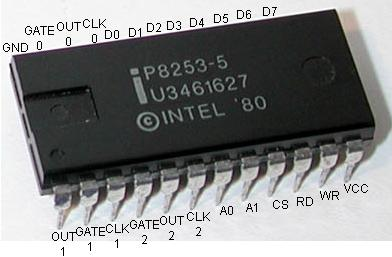
\includegraphics[width=0.5\textwidth]{../img/Intel-P8253-5}
\end{figure}

\subsection{برمجة المؤقتة \en{PIT}}
مؤخراً تم نقل المؤقتة من اللوحة الأم (\en{MotherBoard}) كشريحة \en{DIP} مستلقة الى الجسر الشمالي (\en{SouthBridge}). وسوف نركز على برمجة العداد الأول وهو مؤقت النظام حيث أنه يوفر الدعم العتادي اللازم للنظام حتى يدعم تعدد العمليات والمسالك.

\subsubsection{مشابك المؤقتة \en{PIT's Pins}}
\begin{wrapfigure}{l}{0.5\textwidth}
\label{fig:pit_pins} 
  \vspace{-20pt}
  \begin{center}
    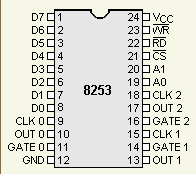
\includegraphics[width=0.48\textwidth]{../img/pit_pins}
  \end{center}
  \vspace{-20pt}
  \caption{مشابك المؤقتة \en{PIT}}
  \vspace{-10pt}
\end{wrapfigure}
تُرسَل الأوامر والبيانات الى المؤقتة وذلك عبر مسار البيانات (\en{Data Bus}) حيث يرتبط هذا المسار مع مشابك البيانات في المؤقتة وهي 8 مشابك \en{D0...D7} وتُمثل 8 بتات. وعند إرسال بيانات الى المؤقتة (عملية كتابة) فان مشبك الكتابة \en{WR} يأخذ قيمة منخفضة دلالة على أن هناك عملية إرسال بيانات الى المؤقتة وكذلك في حالة قراءة بيانات من المؤقتة فإن مشبك القراءة \en{RD} يأخذ قيمة منخفضة دلالة على أن هناك عملية قراءة من المؤقتة. ويتحكم في مشبك القراءة والكتابة مشبك \en{CS} حيث تحدد قيمته تعطيل أو تفعيل عمل الشبكين السابقين ، ويرتبط مشبك \en{CS} مع مسار العناوين (\en{Address Bus}) بينما يرتبط مشبك القراءة والكتابة مع مسار التحكم (\en{Control Bus}). وتُحدد قيمة المشبكين \en{A0,A1} -واللذان يرتبطان مع مسار العنواين- المسجلات المطلوب الوصول اليها داخل المؤقتة. أما المشابك (\en{CLK, OUT, and GATE}) فهي لكل عداد بداخل المؤقتة أي بمعنى أنه توجد ثلاث مشابك من كل واحدة منهم ، ويعتبر المشبكين (\en{CLK (Clock Input) and GATE}) مشابك إدخال للعداد بينما المشبك (\en{OUT}) مشبك إخراج حيث يستخدم لربط العداد مع العتاد فمثلا مشبك الإخراج في العداد الأول (مؤقتة النظام) يرتبط مع متحكم \en{PIC} حيث من خلاله تستطيع مؤقتة النظام إرسال طلب المقاطعة (\en{IRQ0}) الى متحكم \en{PIC} والذي يقوم بتحويل الطلب الى المعالج لكي ينفذ دالة التخديم.

\subsubsection{مسجلات المؤقتة \en{PIT}}
توجد 4 مسجلات بداخل المؤقتة \en{PIT} ، ثلاث منها تستخدم للعدادات (الأول والثاني والثالث) حيث من خلالها يمكن قراءة قيمة العداد أو الكتابة فيه ، وطول مسجل العداد هو 16 بت . وبسبب أن مشابك البيانات التي تربط المؤقتة ومسار البيانات هي من الطول 8 بت فانه لن نتمكن من إرسال البيانات بهذ الشكل . لذلك يجب إستخدام مسجل اخر وهو مسجل التحكم (\en{Control Word}) بحيث قبل إرسال بيانات أو قراءة بيانات من أي عداد فانه يجب إرسال الأمر المطلوب الى مسجل التحكم وبعد ذلك يتم إرسال البيانات أو قرائتها. والجدول \ref{tbl:pit} يوضح هذا المسجلات وعنوان منافذ الإدخال والإخراج المستخدمة للتعامل معها ، ويجب ملاحظة قيم خط القراءة والكتابة وخط العنوان (\en{A0,A1}) حيث تؤثر قيمهم في تحديد نوع العملية المطلوبة (قراءة أم كتابة ورقم العداد).
\begin{table}[h!]
\caption{مسجلات المؤقتة \en{8253 PIT}}
\centering
\begin{tabular}{ | r | r | r | r | r | r | r |}
\hline  
 اسم المسجل & رقم المنفذ & خط \en{RD} & خط \en{WR} & خط \en{A0} & خط \en{A1} & الوظيفة   \\
\hline \hline
\en{Counter 0} & \en{0x40} & \en{1} & \en{0} & \en{0} & \en{0} & كتابة الى المسجل \en{0} \\
 & & \en{0} & \en{1} & \en{0} & \en{0} & قراءة المسجل \en{0} \\
 \hline 
\en{Counter 1} & \en{0x41} & \en{1} & \en{0} & \en{0} & \en{1} & كتابة الى المسجل \en{1} \\
  &   & \en{0} & \en{1} & \en{0} & \en{1} & قراءة المسجل \en{1} \\
 \hline 
\en{Counter 2} & \en{0x42} & \en{1} & \en{0} & \en{1} & \en{0} & كتابة الى المسجل \en{2} \\
 &   & \en{0} & \en{1} & \en{1} & \en{0} & قراءة المسجل \en{2} \\
 \hline 
\en{Control Word} & \en{0x43} & \en{1} & \en{0} & \en{1} & \en{1} & كتابة \en{Control Word} \\
  &   & \en{0} & \en{1} & \en{1} & \en{1} & لا توجد عملية \\
 \hline  
\end{tabular}
\label{tbl:pit}
\end{table}
وتوضح التركيبة التالية ماهية البتات المستخدمة في مسجل التحكم (وهو مسجل بطول 8 بت) حيث يجب إرسال قيم معينة حتى نتمكن من القراءة أو الكتابة في عداد ما.
\begin{english}
\fontspec[Scale=1.2,Mapping=englishdigits]{Calibri}

\begin{itemize}
\item  Bit 0: (BCP) Binary Counter
\begin{itemize}
\item  0: Binary
\item  1: Binary Coded Decimal (BCD)
\end{itemize}
\item  Bit 1-3: (M0, M1, M2) Operating Mode. See above sections for a description of each.
\begin{itemize}
\item  000: Mode 0: Interrupt or Terminal Count
\item   001: Mode 1: Programmable one-shot
\item  010: Mode 2: Rate Generator
\item  011: Mode 3: Square Wave Generator
\item  100: Mode 4: Software Triggered Strobe
\item  101: Mode 5: Hardware Triggered Strobe
\item  110: Undefined; Don't use
\item  111: Undefined; Don't use
\end{itemize}
\item   Bits 4-5: (RL0, RL1) Read/Load Mode. We are going to read or send data to a counter register
\begin{itemize}
\item  00: Counter value is latched into an internal control register at the time of the I/O write operation.
\item   01: Read or Load Least Significant Byte (LSB) only
\item  10: Read or Load Most Significant Byte (MSB) only
\item  11: Read or Load LSB first then MSB
\end{itemize}
\item  Bits 6-7: (SC0-SC1) Select Counter. See above sections for a description of each.
\begin{itemize}
\item   00: Counter 0
\item  01: Counter 1
\item  10: Counter 2
\item  11: Illegal value
\end{itemize}

\end{itemize}
\end{english}

والمثال \ref{lst:timer} يوضح كيفية برمجة عداد مؤقت النظام لإرسال طلب مقاطعة كل \en{100Hz} (كل 10 \en{milliseconds}) ، وهذا يتم عن طريق إرسال أمر التحكم أولاً ومن ثم إرسال الوقت المطلوب الى العداد المطلوب.

\begin{english}
\fontspec{Courier New}

\lstset{numberstyle=\tiny,numbers=left,stepnumber=1,numbersep=5pt,tabsize=2,extendedchars=true,breaklines=true,frame=b,showspaces=false, showtabs=false,xleftmargin=10pt,framexleftmargin=10pt,framexrightmargin=5pt,framexbottommargin=4pt,showstringspaces=false,language=[x86masm]Assembler}


\begin{lstlisting}[label=lst:timer,caption=\en{PIT programming}]
       ; COUNT = input hz / frequency
 
	mov	dx, 1193180 / 100	; 100hz, or 10 milliseconds
 
	; FIRST send the command word to the PIT. Sets binary counting,
	; Mode 3, Read or Load LSB first then MSB, Channel 0
 
	mov	al, 110110b
	out	0x43, al
 
	; Now we can write to channel 0. Because we set the "Load LSB first then MSB" bit, that is
	; the way we send it
 
	mov	ax, dx
	out	0x40, al	;LSB
	xchg	ah, al
	out	0x40, al	;MSB
\end{lstlisting}
\end{english}

\end{document}